\DiaryEntry{Lossless Compression and Huffman Code}{2021-04-14}{Coding}

\subsection{Introduction}

Coding (here) means the assignment of binary sequences to elements of an alphabet. The set of binary sequences is called a code, and the individual members of the set are called codewords. An alphabet is a collection of symbols called letters.

As an example, the ASCII code for 'A' is $65$ which corresponds to $01000001$ in binary notation. ASCII is an example of a \emph{fixed-width} code where every codeword has the same bitlength.

If we want to reduce the number of bits required to represent different symbols, we need to use a different number of bits to represent different symbols. If we use fewer bits to represent elements that occur more often, on the average we would use fewer bits per symbol. The average number of bits per symbol is often called the rate of the code.

We denote the symbols as $a_i$ and their probability with $P(a_i)$. If each codeword $a_i$ is represented with $n(a_i)$ bits, the average length $l$ is given bayes

\bee
l = \sum_i P(a_i) n(a_i)
\eee

\paragraph{Code Properties.} In the following, we consider $4$ different codes which illustrate different properties of codes.

\vspace{3mm}

\begin{tabular}{c|cccc}
    \label{2021-04-14_tab1}
    Symbol & Code 1 & Code 2 & Code 3 & Code 4 \\ \hline
    $a_1$ & 0 & 0 & 0 & 0  \\
    $a_2$ & 0 & 1 & 10 & 01  \\
    $a_3$ & 1 & 00 & 110 & 011  \\
    $a_4$ & 10 & 11 & 111 & 0111
\end{tabular}

\vspace{3mm}

Code 1 cannot be unambiguously decoded as $a_1$ and $a_2$ have the same binary representation. When $a_0$ is received, there is no way to know whether an $a_1$ was transmitted or an $a_2$. We would like each symbol to be assigned a \emph{unique} codeword.

Code 2 is better in the sense that all codewords are different. However, assume we receive the binary sequence $00$: Then it is not clear whether this corresponds to the sequence $a_1 a_1$ or $a_3$. Once a sequence is encoded with Code 2, the original sequence cannot be recovered with certainty. In general, this is not a desirable property for a code. We would like \emph{unique decodability} from the code; that is, any given sequence of codewords can be decoded in one, and only one, way.

With Code 3, we notice that the first three codewords all end in a $0$. In fact, a $0$ always denotes the termination of a codeword. The final codeword contains no $0$s and is $3$ bits long. Because all other codewords have fewer than three $1$s and terminate in a $0$, the only way we can get three 1s in a row is as a code for $a_4$ . The decoding rule is simple. Accumulate bits until you get a $0$ or until you have three $1$s. There is no ambiguity in this rule, and it is reasonably easy to see that this code is uniquely decodable.

With Code 4 we have an even simpler condition. Each codeword starts with a $0$, and the only time we see a $0$ is in the beginning of a codeword. Therefore, the decoding rule is to accumulate bits until you see a $0$. The bit before the 0 is the last bit of the previous codeword.

There is a slight difference between Code 3 and Code 4. In the case of Code 3, the decoder knows the moment a code is complete. In Code 4, we have to wait till the beginning of the next codeword before we know that the current codeword is complete. Because of this property, Code 3 is called an \emph{instantaneous code}. Although Code 4 is not an instantaneous code, it is almost that.

While this property of instantaneous or near-instantaneous decoding is a nice property to have, it is not a requirement for unique decodability. Consider the code shown in the table below. Let’s decode the string $011111111111111111$. In this string, the first codeword is either $0$ corresponding to $a_1$ or $01$ corresponding to $a_2$ . We cannot tell which one until we have decoded the whole string. Starting with the assumption that the first codeword corresponds to $a_1$ , the next eight pairs of bits are decoded as $a_3$. However, after decoding eight $a_3$s, we are left with a single (dangling) $1$ that does not correspond to any codeword. On the other hand, if we assume the first codeword corresponds to $a_2$, we can decode the next $16$ bits as a sequence of eight $a_3$s; and we do not have any bits left over. The string can be uniquely decoded. In fact, Code 5, while it is certainly not instantaneous, is uniquely decodable.

\vspace{3mm}

\begin{tabular}{c|c}
    Symbol & Code 5 \\ \hline
    $a_1$ & 0 \\
    $a_2$ & 01 \\
    $a_3$ & 11
\end{tabular}

\vspace{3mm}

In the last example, we found that we had an incorrect decoding because we were left with a binary string ($1$) that was not a codeword. If this had not happened, we would have had two valid decodings.

Such a case is shown in the following exmaple.

\vspace{3mm}

\begin{tabular}{c|c}
    Symbol & Code 5 \\ \hline
    $a_1$ & 0 \\
    $a_2$ & 01 \\
    $a_3$ & 10
\end{tabular}

\vspace{3mm}

Let’s encode the sequence $a_1$ followed by eight $a_3$s using this code. The coded sequence is $01010101010101010$. The first bit is the codeword for $a_1$. However, we can also decode it as the first bit of the codeword for $a_2$ . If we use this (incorrect) decoding, we decode the next seven pairs of bits as the codewords for $a_2$. After decoding seven $a_2$s, we are left with a single $0$ that we decode as $a_1$. Thus, the incorrect decoding is also a valid decoding, and this code is not uniquely decodable.


\paragraph{Unique Decodability.} In the previous examples, in the case of the uniquely decodable code, the binary string left over after we had gone through an incorrect decoding was not a codeword. In the case of the code that was not uniquely decodable, in the incorrect decoding what was left was a valid codeword. Based on whether the dangling suffix is a codeword or not, we get the following test.

Suppose we have two binary codewords $a$ and $b$, where $a$ is $k$ bits long, $b$ is $n$ bits long, and $k < n$. If the first $k$ bits of $b$ are identical to $a$, then $a$ is called a prefix of $b$. The last $n - k$ bits of $b$ are called the dangling suffix. For example, if $a = 010$ and b = $01011$, then $a$ is a prefix of $b$ and the dangling suffix is $11$.

Thje procedure for deciding unique decoability is as follows: Construct a list of all the codewords. Examine all pairs of codewords to see if any codeword is a prefix of another codeword. Whenever you find such a pair, add the dangling suffix to the list unless you have added the same dangling suffix to the list in a previous iteration. Now repeat the procedure using this larger list. Continue in this fashion until one of the following two things happens: 1. You get a dangling suffix that is a codeword. 2. There are no more unique dangling suffixes.

If you get the first outcome, the code is not uniquely decodable. However, if you get the second out- come, the code is uniquely decodable.

\paragraph{Prefix Codes.} The test for unique decodability requires examining the dangling suffixes initially generated by code-word pairs in which one codeword is the prefix of the other. If the dangling suffix is itself a codeword, then the code is not uniquely decodable. One type of code in which we will never face the possibility of a dangling suffix being a codeword is a code in which no codeword is a prefix of the other. In this case, the set of dangling suffixes is the null set, and we do not have to worry about finding a dangling suffix that is identical to a codeword. A code in which no codeword is a prefix to another codeword is called a \emph{prefix code}. A simple way to check if a code is a prefix code is to draw the rooted binary tree corresponding to the code. Draw a tree that starts from a single node (the root node) and has a maximum of two possible branches at each node. One of these branches corresponds to a $1$ and the other branch corresponds to a $0$. By convention, when we draw a tree with the root node at the top, the left branch corresponds to a $0$ and the right branch corresponds to a $1$. Using this convention, we can draw the binary tree for Code 2, Code 3, and Code 4 as shown in the following Figure.

\begin{figure}[H]
    \centering
    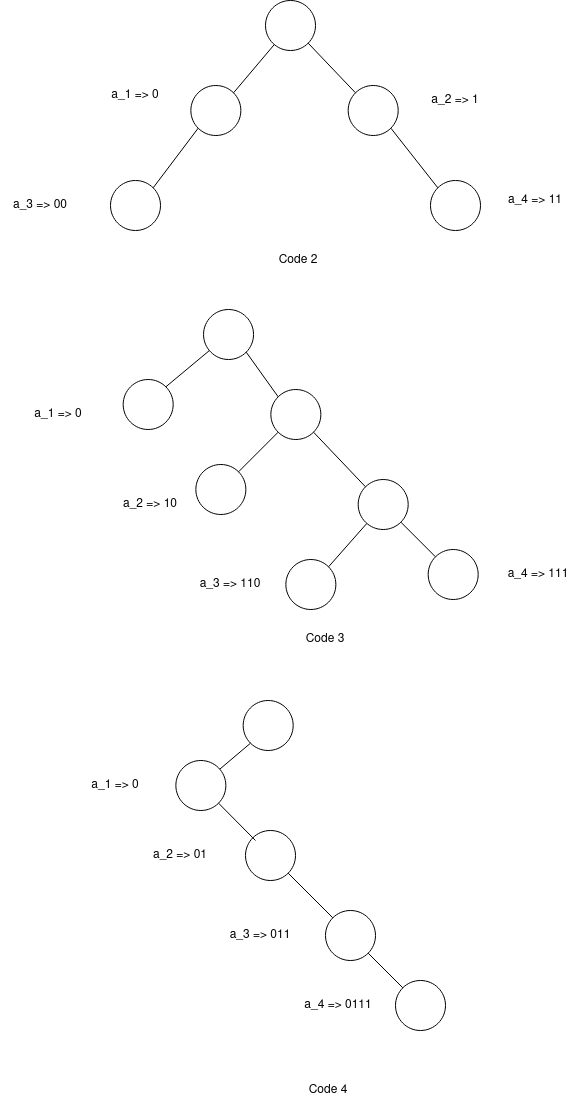
\includegraphics[scale=0.4]{images/2021-04-14-tree.png}
\end{figure}

Note that apart from the root node, the trees have two kinds of nodes—nodes that give rise to other nodes and nodes that do not. The first kind of nodes are called \emph{internal nodes}, and the second kind are called \emph{external nodes} or \emph{leaves}. In a prefix code, the codewords are only associated with the external nodes. A code that is not a prefix code, such as Code 4, will have codewords associated with internal nodes. The code for any symbol can be obtained by traversing the tree from the root to the external node corresponding to that symbol. Each branch on the way contributes a bit to the codeword: a 0 for each left branch and a 1 for each right branch.

It is nice to have a class of codes, whose members are so clearly uniquely decodable. However, are we losing something if we restrict ourselves to prefix codes? Could it be that if we do not restrict ourselves to prefix codes, we can find shorter codes? Fortunately for us the answer is no. For any nonprefix uniquely decodable code, we can always find a prefix code with the same codeword lengths.

\paragraph{Kraft-McMillian Inequality.} It's actually two parts. First we have a necessary condition on the codeword length of uniquely decodable codes.

\begin{theorem}
    Let $\Cc$ be a code with $N$ codewords of length $l_1, l_2, \ldots, l_N$. If $\Cc$ is uniquely decodable, then

    \bee
        K(\Cc) = \sum_i 2^{-l_i} \leq 1
    \eee
\end{theorem}

Proof is omitted.

The second part is that if we have a code fulfilling the condition above, then there exists a prefix code with the given codelengths.

\begin{theorem}
    Given a set of integers $l_1, l_2, \ldots, l_N$ fulfilling

    \bee
        K(\Cc) = \sum_i 2^{-l_i} \leq 1
    \eee

    then we can always find a prefix code with codeword lengths $l_1, l_2, \ldots, l_N$.
\end{theorem}

Proof is omitted.

To summarize, if we have a uniquely decodable code, the codeword lengths have to satisfy the Kraft– McMillan inequality. If we are given codeword lengths that satisfy the Kraft–McMillan inequality, we can always find a prefix code with those codeword lengths. Thus, by restricting ourselves to prefix codes, we are not in danger of overlooking nonprefix uniquely decodable codes that have a shorter average length.

\subsection{Huffman Codes}

The Huffman procedure is based on two observations regarding optimum prefix codes. 

\begin{itemize}
    \item In an optimum code, symbols that occur more frequently (have a higher probability of occurrence) will have shorter codewords than symbols that occur less frequently.
    
    \item  In an optimum code, the two symbols that occur least frequently will have the same length.
\end{itemize}


 The first observation is rather straightforward: If symbols that occur more often had codewords that were longer than the codewords for symbols that occurred less often, the average number of bits per symbol would be larger than if the conditions were reversed. Therefore, a code that assigns longer codewords to symbols that occur more frequently cannot be optimum.
 
 To see why the second observation holds true, consider the following situation. Suppose an optimum code exists in which the two codewords corresponding to the two least probable symbols do not have the same length. Suppose the longer codeword is $k$ bits longer than the shorter codeword. Because this is a prefix code, the shorter codeword cannot be a prefix of the longer codeword. This means that even if we drop the last $k$ bits of the longer codeword, the two codewords would still be distinct. As these codewords correspond to the least probable symbols in the alphabet, no other codeword can be longer than these codewords (by observation 1); therefore, there is no danger that the shortened codeword would become the prefix of some other codeword. Furthermore, by dropping these $k$ bits we obtain a new code that has a shorter average length than $\Cc$. But this violates our initial contention that $\Cc$ is an optimal code. Therefore, for an optimal code the second observation also holds true.

 The Huffman procedure adds a simple requirement to these two observations. This requirement is that the codewords corresponding to the two lowest probability symbols differ only in the last bit. Assume that $a$ and $b$ are the two least probable symbols in an alphabet. If the codeword for $b$ is $m+0$, the codeword for $b$ would be $m + 1$. Here, $m$ is a string of $1$s and $0$s; and $+$ denotes concatenation. This requirement does not violate our two observations and leads to a very simple encoding procedure.

\paragraph{Code Construction.} The following Figure shows the Huffman code construction with an example. We have $N = 5$ symbols; the symbols and their probabilities are shown on the left with red background. The algorithm starts by combining the two symbols with the lowest probability, that is symbol $1$ and symbol $2$. Their combined probability is $0.08 + 0.1 = 0.18$ which is combined with symbol $3$. We arrive at a probability of $0.12 + 0.18 = 0.3$, combine with symbol $4$, get a probability of $0.3 + 0.25 = 0.55$, and finally combine with symbol $5$ (having probability $1.0$ as we have combined all symbols together).

\begin{figure}[H]
    \centering
    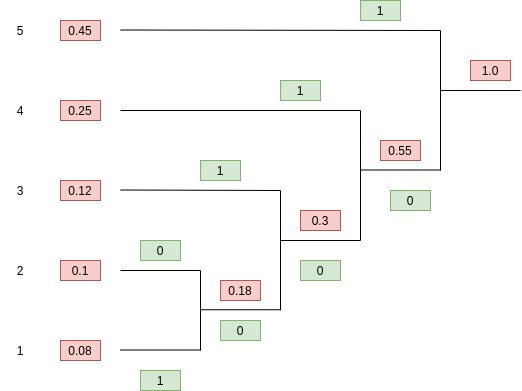
\includegraphics[scale=0.5]{images/2021-04-14-code_1.png}
\end{figure}

To get to the binary labels of the symbols, we walk our way backwards in the tree; the symbol with the higher probability gets a $0$, the other a $1$. They are shown with green background in the Figure. We read off the binary label from right to left. In this case, we arrive at the following labels.

\vspace{3mm}

\begin{tabular}{cc|c}
    Symbol & Probability & Codeword \\ \hline
    $1$ & $0.08$ & $0001$ \\
    $2$ & $0.1$ & $0000$ \\
    $3$ & $0.12$ & $001$ \\
    $4$ & $0.25$ & $01$ \\
    $5$ & $0.45$ & $1$
\end{tabular}

\vspace{3mm}

The average code length is given according to

\bee
l = 0.08 \cdot 4 + 0.1 \cdot 4 + 0.12 \cdot 3 + 0.25 \cdot 2 + 0.45 \cdot 1 = 2.03 \text{bits/Symbol}
\eee

The source entropy is approximately, $2.01$ bits / symbol, so the Huffman code comes quite close.

Actually, the example is slightly biased as representing $5$ symbols with a fixed-length code requires $3$ bits and therefore $2^3 - 5 = 3$ symbols is wasted. The fixed length code has (by definition) an average code length of $3$, so by using a Huffman code we save almost $1$ bit!

As another example, consider the following Huffman code construction with $N = 8$. Note that always the two symbols with the lowest probability are combined; after we have combined symbol $4$, the two smallest symbols are symbol $5$ and $6$ which are therefore combined next. In addition, there is some ambiguity when assigning bits to the tree; e.g. when deciding at the beginning of the tree there are two sybols with probability $0.5$ each. In a similar spirit, there is an ambiguity between symbols $5$ and $6$.

\begin{figure}[H]
    \centering
    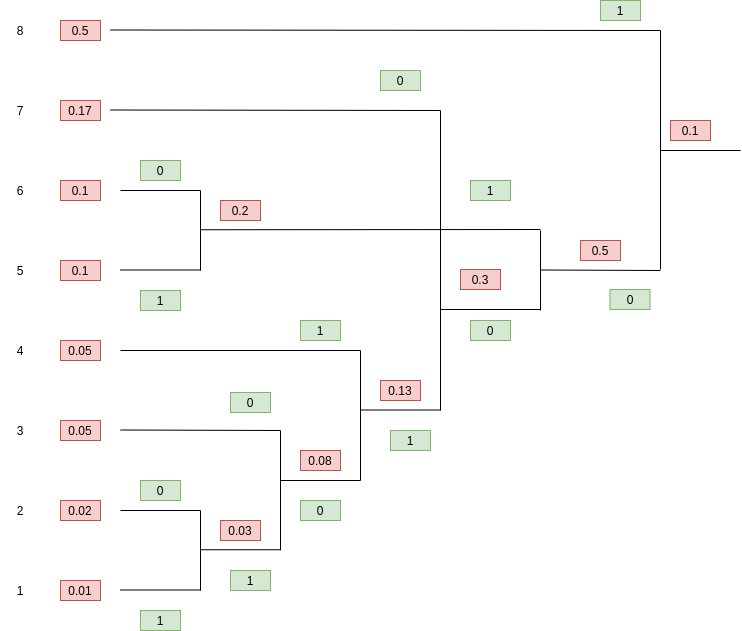
\includegraphics[scale=0.5]{images/2021-04-14-code_2.png}
\end{figure}

I have written a Julia file which creates a Huffmann code given symbols with probabilities. This one producesa Huffmann code slightly different than the construction above; however, the assigned code word lengths are the same. This yields an average code length of $l = 2.24$ bits / Symbol. Comparing to the fixed-length code which requires $\log_2 8 = 3$ bits / Symbol, we still have significant savings. Compared with the source entropy of $2.21$ bits / Symbol, the Huffman code achieves good performance.



%%% Local Variables:
%%% mode: latex
%%% TeX-master: "journal"
%%% End:
